\section*{Lecture 24}

\subsection*{1.} Calculate the rotation of
\[ 
  \Vec{v} \left( x,y,z \right) = \left( \frac{y}{z^2}, \frac{z}{x^2}, \frac{x}{y^2} \right) 
.\]
\bigbreak
The rotation is defined as:
\[ 
\nabla \times \Vec{v}(x,y,z) = \left| \begin{array}{ccc}
\Vec{i} & \Vec{j} & \Vec{kj}\\
\frac{\partial }{\partial x} & \frac{\partial }{\partial y} & \frac{\partial }{\partial z}\\
\frac{y}{z^2} & \frac{z}{x^2} & \frac{x}{y^2}\\
\end{array} \right|
.\]
Which gives us:
\begin{align*}
 \left| \begin{array}{ccc}
\Vec{i} & \Vec{j} & \Vec{k}\\
\frac{\partial }{\partial x} & \frac{\partial }{\partial y} & \frac{\partial }{\partial z}\\
\frac{y}{z^2} & \frac{z}{x^2} & \frac{x}{y^2}\\
\end{array} \right| &= \Vec{i} \left( -2 \frac{x}{y^3} - \frac{1}{x^2} \right) - \Vec{j} \left( \frac{1}{y^2} + 2 \frac{y}{z^3} \right) + \Vec{k} \left( - 2 \frac{z}{x^3} - \frac{1}{z^2} \right) \\
&= \left( -2\frac{x}{y^3} - \frac{1}{x^2}, - \frac{1}{y^2} - 2 \frac{y}{z^3}, -2 \frac{z}{x^3} - \frac{1}{z^2} \right)
.\end{align*}

\subsection*{2.} Let $f \left( x,y,z \right) , g(x,y,z)$ be scalar fields and $\Vec{v}(x,y,z), \Vec{w}(x,y,z)$ be vector fields. Do the following expressions make sense?

\paragraph{(a)}
\[ 
\mathrm{rot}\left( \Vec{w}(x,y,z) + \mathrm{grad}\left( \mathrm{div}\left( f(x,y,z) \Vec{v}\left( x,y,z \right) \right) \right)  \right) 
.\]
\bigbreak
We start from the inside.
\begin{itemize}
  \item $f \Vec{v}$ makes sense and gives a vector field
  \item $\mathrm{div}(f \Vec{v})$ is the divergence of a vector field which gives a scalar field
  \item $\mathrm{grad}(\mathrm{div}(f \Vec{v}))$ is the gradient of a scalar field which gives a vector field
  \item $\Vec{w} + \mathrm{grad}(\mathrm{div}(f \Vec{v}))$ is the sum of two vector field giving a vector field
  \item $\mathrm{rot}\left( \Vec{w} + \mathrm{grad} \left( \mathrm{div} \left( f \Vec{v} \right) \right) \right)$ is the rotation of a vector field which makes sense
\end{itemize}

\paragraph{(b)}
\[ 
\mathrm{grad}\left( \left( \Vec{v} \left( x,y,z \right) \cdot \Vec{w}\left( x,y,z \right)  \right) + \mathrm{div} \left( \mathrm{grad} \left( f \left( x,y,z \right) \left( \Vec{v} \left( x,y,z \right) \cdot \Vec{v} \left( x,y,z \right)  \right)  \right)  \right)  \right) 
.\]
\bigbreak
We again start from the inside.
\begin{itemize}
  \item $\Vec{v} \cdot \Vec{v}$ and $\Vec{v} \cdot \Vec{w}$ both make sense and give scalar fields
  \item $f (\Vec{v} \cdot \Vec{v})$ is a scalar field multiplied by a scalar field which gives a scalar field
  \item $\mathrm{grad}\left( f \left( \Vec{v} \cdot \Vec{v} \right) \right)$ is the gradient of a scalar field which gives a vector field
  \item $\mathrm{div} \left( \mathrm{grad} \left( f \left( \Vec{v} \cdot \Vec{v} \right) \right) \right)$ is the divergence of a vector field which gives a scalar field
  \item $\left( \Vec{v} \cdot \Vec{w} \right) + \left( \mathrm{div} \left( \mathrm{grad}\left( f \left( \Vec{v}\cdot \Vec{v} \right) \right) \right) \right)$ is the sum of two scalar fields which gives a scalar field
  \item $\mathrm{grad} \left( \left( \Vec{v} + \Vec{w} \right) + \mathrm{div} \left( \mathrm{grad} \left( f \left( \Vec{v}\cdot \Vec{v} \right) \right) \right) \right)$ is the gradient of a scalar field which gives a vector field
\end{itemize}

\paragraph{(c)}
\[ 
\mathrm{rot}\left( \Vec{w}\left( x,y,z \right) + \mathrm{grad}\left( \mathrm{div}\left( f \left( x,y,z \right) + \Vec{v}\left( x,y,z \right)  \right)  \right)  \right) 
.\]
\bigbreak
If we start from the middle we see that $f + \Vec{v}$ does not make sense.

\paragraph{(d)}
\[ 
\mathrm{grad} \left( \left( \Vec{v}\left( x,y,z \right) \cdot \Vec{w}\left( x,y,z \right)  \right) + \mathrm{div}\left( \mathrm{grad}\left( \Vec{w}\left( x,y,z \right) \left( \Vec{v}\left( x,y,z \right) \cdot \Vec{v}\left( x,y,z \right)  \right)  \right)  \right)  \right) 
.\]
\bigbreak
Once again, we start from the middle.
\begin{itemize}
  \item $\Vec{v} \cdot \Vec{v}$ makes sense and gives a scalar field
  \item $\Vec{w}\left( \Vec{v}\cdot \Vec{v} \right)$ gives a vector field
  \item $\mathrm{grad}\left( \Vec{w}\left( \Vec{v}\cdot \Vec{v} \right) \right) $ is the gradient of a vector field, which gives a tensor field, which is not covered in the course and therefore does not make sense in this context.
\end{itemize}


\subsection*{3.} Let
\[ 
\Vec{F} \left( \Vec{r} \right) = \left( x^2, z^2, y^2 \right) 
.\]
Consider the curve
\[ 
C: \Vec{r}(t) = \left( 0,t, |t| \right) \qquad -1 \leq t \leq 1
.\]

\paragraph{(a)} Sketch the curve $C$.
\bigbreak
\begin{figure} [ht]
  \centering
  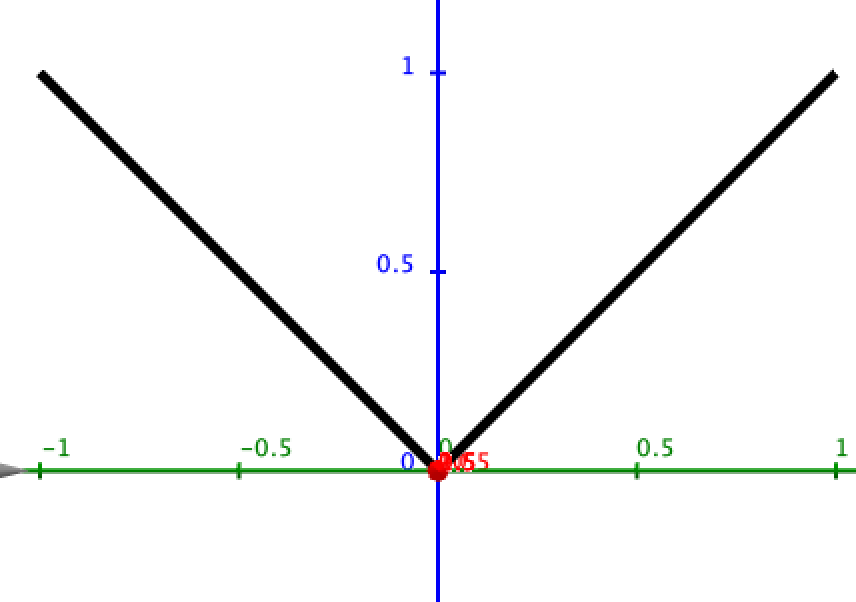
\includegraphics[width=0.5\linewidth]{./figures/f24_1.png}
  \caption{The curve $C$ in the $yz$-plane ($x=0$)}
  \label{fig:f24_1}
\end{figure}

\paragraph{(b)} Calculate $\int_{C} \Vec{F} \left( \Vec{r} \right) \cdot \, \mathrm{d}\Vec{r}$.
\bigbreak
The tangent $\Vec{r}'(t)$ for $0 t \leq 1$ is:
\[ 
\Vec{r}'(t) = (0, t, t)' = (0,1,1)
.\]
The tangent $\Vec{r}'(t)$ for $-1 \leq t < 0$ is:
\[ 
\Vec{r}'(t) = (0, t, -t) = (0, 1, -1)
.\]
The scalar product $\Vec{F}\left( \Vec{r}(t) \right)\cdot \Vec{r}'(t)$ is therefore
\begin{align*}
  \text{For }0 \leq t \leq 1 &: 2t^2 \\
  \text{For } -1 \leq t \leq 0 &: 0
.\end{align*}
Therefore the line integral is:
\begin{align*}
  \int_{C} \Vec{F} \left( \Vec{r} \right) \, \mathrm{d}\Vec{r} &= \int_{-1}^{1} \Vec{F} \left( \Vec{r}(t) \right)\cdot \Vec{r}'(t) \, \mathrm{d}t \\
  &= \int_{-1}^{0} \Vec{F} \left( \Vec{r}(t) \right) \Vec{r}'(t) \, \mathrm{d}t + \int_{0}^{1} \Vec{F} \left( \Vec{r}(t) \right) \Vec{r}'(t) \\
  &= \int_{0}^{1} 2t^2 \, \mathrm{d}t \\
  &= 2 \left[ \frac{t^3}{3} \right]_{0}^{1} \\
  &= \frac{2}{3}
.\end{align*}



\subsection*{4.} Find $f(\Vec{r})$ such that $\Vec{F}\left( \Vec{r} \right) = \nabla f \left( \Vec{r} \right) $ and calculate the line integral along the curve
\[ 
C : \Vec{r}(t) = \left( e^{t}, \cos t, \sin t \right), 0 \leq t \leq \frac{\pi}{2}
\]
for

\paragraph{(a)} $\Vec{F}(\Vec{r}) = \left( yz, xz, xy \right)$.
\bigbreak
We calculate the scalar field as:
\begin{align*}
  \Vec{F}(x,y,z) &= \nabla f(x,y,z) \\
  \implies F_1(x,y,z) &= \frac{\partial f(x,y,z)}{\partial x} \\
  F_2(x,y,z) &= \frac{\partial f(x,y,z)}{\partial y} \\
  F_3(x,y,z) &= \frac{\partial f(x,y,z)}{\partial z}
.\end{align*}
The first equation gives us that:
\begin{align*}
  F_1 (x,y,z) &= \frac{\partial f(x,y,z)}{\partial x} \\
  \implies yz &= \frac{\partial \frac{f}{x,y,z)}}{\partial \frac{\partial x}{\partial }} \\
  \implies f(x,y,z) &= xyz + g(y,z)
.\end{align*}
The second equation gives:
\begin{align*}
  F_2(x,y,z) &= \frac{\partial f(x,y,z)}{\partial y} \\
  \implies xz &= xz + \frac{\partial g(y,z)}{\partial y} \\
\implies g(y,z) &= g(z) \\
\implies f(x,y,z) = xyz + g(z)
.\end{align*}
And likewise the third equation gives:
\begin{align*}
  F_3(x,y,z) &= \frac{\partial f(x,y,z)}{\partial z} \\
  \implies xy &= xy + \frac{\partial g(z)}{\partial z} \\
  \implies g(z) &= \mathrm{const}
.\end{align*}
We choose $g(z) = 0 \implies f(x,y,z) = xyz$ and get the line integral:
\[ 
\int_{C} \Vec{F} (\Vec{r})\cdot \, \mathrm{d}\Vec{r} = f \left( \Vec{r} \left( \frac{\pi}{2} \right) \right) - f(\Vec{r}(0)) = e^{\frac{\pi}{2}} \cos \frac{\pi}{2} \sin \frac{\pi}{2} - e^{0} \cos 0 \sin 0 = 0
.\]



\paragraph{(b)} $\Vec{F}\left( \Vec{r} \right) = \left( y^2 + 2xz, 2xy + z^2, 2yz + x^2 \right) $.
\bigbreak
This time the three equations gives:
\begin{align*}
  y^2 + 2xz &= \frac{\partial f(x,y,z)}{\partial x} \\
  \implies f(x,y,z) &= xy^2 + x^2z + g(y,z) \\
  2xy + z^2 &= 2xy + \frac{\partial g(y,z)}{\partial y} \\
  \implies g(y,z) &= yz^2 + h(z) \\
  \implies f(x,y,z) &= xy^2 + zx^2 + yz^2 + h(z) \\
  2yz + x^2 &= x^2 + 2yz + \frac{\partial h(z)}{\partial z} \\
  \implies h(z) &= \mathrm{const} \\
.\end{align*}
We choose $h(z) = 0 \implies f(x,y,z) = xy^2 + zx^2 + yz^2$. This gives the line integral:
\[ 
\int_{C} \Vec{F} \left( \Vec{r} \right) \, \mathrm{d}\Vec{r} = f \left( \Vec{r} \left( \frac{\pi}{2} \right) \right) - f \left( \Vec{r}(0) \right) = e^{\frac{\pi}{2}} \cos^2 \frac{\pi}{2} + \sin \frac{\pi}{2} e^{\pi} + \cos \frac{\pi}{2} \sin^2 \frac{\pi}{2} = e^{\pi} - 1
.\]

